\documentclass[12pt,oneside]{book}
\usepackage{preamble}
%\setuptodonotes{disable}

\begin{document}
\begin{titlepage}\centering
    \begin{figure}[ht!]\centering
\includegraphics{img/bruni-logo.png}\end{figure}
    \vfill\textbf{\Huge Playing the Periphery}\vspace{24mm}\\
    {\huge A thesis submitted for the degree of\\MA Games Design\\
    \vspace{8mm}by}\vspace{8mm}\\\texttt{\LARGE 2\>4\>4\>1\>8\>7\>1}\vfill
    {\Large Department of Arts and Humanities, Brunel University London}
\end{titlepage}

\newgeometry{margin=12mm}
\tableofcontents
\begingroup\let\clearpage\relax\listoffigures\endgroup
\restoregeometry

\newgeometry{top=16mm,bottom=16mm}
\chapter*{Abstract}\addcontentsline{toc}{section}{\textit{Abstract}}
\begin{center}\begin{singlespace}\vspace{-4mm}
    \todo[add,noinline]{refresh abstract}
    My topic of interest lies at the intersection of paratextual, corporeal, and sociocultural aspects of iconic game titles and their impact of their legacy.
    In other words, elements that lie at and/or outside the perimeter of the magic circle \parencite{huizinga}.
    Paratext consists of surrounding media not included in the game itself but strongly influencing how the experience is accessed, framed, and understood.
    Material comprises the physical means and contexts of play, in turn shaping the experience through sensory input, physical feedback, and presence. 
    Community is embodied by the players themselves through shared habits, beliefs, and informal systems.
    The synergy of this trinity is flavoured by the aesthetics of the game playing experience in its entirety.
    Moreover, pairing any of these three permeates another facet of that external conceptual space.\par
    In consideration of these angles, my project poses the following question:
    \begin{displayquote}
        \textbf{\textit{In what ways can contemporary game design achieve holistic aesthetic experiences in the likeness of historically acclaimed game titles?}}
    \end{displayquote}
    The research perspective is mostly aimed at context awareness and experiential revision, although, nostalgia remains a latent yet potent factor that bears investigation.
    Retrospective settings are being highlighted because most well-known titles from the past represent history as written by the victors.\footnote{Or, in a few amusingly infamous cases, the kitschy underdogs and dark horses that are often both cautionary tales and subjects of cult following. Evidently, if one struggles to attain immortality via glory, becoming an anecdote remains a viable alternative.}
    With this in mind, I believe that game design can notably benefit from closely examining the external circumstances which frame any media product's release.\par
    The theoretical research will examine existing frameworks established in game and media fields of study, intending to touch on fields and concepts such as 
    experiential aesthetics, affect theory, procedural rhetoric, immersion, metagaming, preservation, and various design approaches.
    The practical review will survey an assortment of games whose play experience is notably characterised by contextual circumstances.
    This investigation is meant to derive patterns from exemplary case studies that can suggest ways of implanting the external layers of play experience into a new piece of playable media.
    With historical awareness providing the background, some of the findings will be incorporated into designing a digital artifact complementing the written one, accompanied by fictional context in the shape of lore and paraphernalia.\par
    Comprehensive analysis of multiple real world scenarios is to be followed by a selection of applicable
    \footnote{A word which here means \parencite{asoue} "feasible".}
    approaches, which in turn will inform the directions taken throughout the design and development process.
    Concurrently, any relevant observations should be recorded with the intent to feed back into the writing and, eventually, provide a strong basis for reflection.
    Exercising theory in practice is expected to direct the unfolding of the game's design.
    The goal that I aspire to achieve with this project is tracing a model of media creation that is elevated by its surrounding context, and also aligns with key values established in my personal game design philosophy \parencite*[GD5609,][]{myDesignPhil}, then put the resulting framework into future practice.
\end{singlespace}\end{center}
\clearpage\restoregeometry\doublespacing

\chapter{Introduction\label{chap:1-intro}}
    \todochap{INTRO}
\section*{Extrinsic Circles}
Contextual influences and overall legacy impact are among the focal points for both primary and secondary sources considered in this paper.
Theoretical examinations will mostly engage with the humanities of game studies - particularly sociocultural and media fields.
Academic texts used as secondary resources range in topic:
 from transtextuality, semiotics, and meta-fiction in media, 
 through platform studies, 
 to sociocultural phenomenology
The research question, however, is more for the benefit of exploring an outside-in perspective on production and design, so it will be supported by practical use cases.
Beside actual video game properties, various technologies (software, hardware, and all in between) are also examined for their contributions.
Nonetheless, those cases will still be illustrated with reference to applicable game titles.

\begin{figure}[ht]
    \tikzperi\caption{Peripheral aspects of play\label{fig:peri-play}}
\end{figure}

When put together, Paratextuality, Physicality, and Popularity can be treated like X/Y/Z axes in a coordinate system. Given any game as a source, evaluating its properties as measures along these axes yields coordinates that denote the facets of paraphernalia, preservation, and personalisation.

The model presented in Figure \ref{fig:peri-play} is by no means indented to contradict or overrule any existing discourse on the matter.
It is solely an amalgamation of theoretical templates and personal pattern recognition assembling a blueprint of my own perspective on the external elements factoring in the periphery of play.

\section*{Premise}
\begin{wrapfigure}{r}{0.2\textheight}\centering
    
\includegraphics[width=0.2\textwidth, height=0.2\textheight]{img/triforce.png}
    \caption[Triforce of play]{Triforce:\\Wisdom, Strength, Courage\\(Nintendo EAD,\cite*{loz-alttp})}
\end{wrapfigure}
I have made the possibly unconventional choice of splitting the practical half of this project further into two games.One has the digital prototype role, while the other is rather a conceptual case study.
The reason for that approach is a matter of positioning.
In order to focus on analysing the outer spaces of gameplay experience, it is almost imperative that the foundation itself is built \textit{outside} said gameplay, with the design \& creation process directed \textit{inwards}.
Keeping in mind the immutable reality of human limitations, a retrospective inquiry at the aesthetic legacy and sociocultural impact of a video game developed by a solo student, on a scale large enough to be of any consequence, is not only an infeasible undertaking, but one that would naturally steer all efforts towards actual development at the expense of design.
Although that would be an achievement of large proportions, it would bring little value towards the purpose of this exercise.
As it turns out, the subject of the case study does not, technically, exist.
At least not in the form of the playable media it is supposed to to represent.
Rather, it shall be defined through negative space, i.e., the silhouette made from all the shapes that are not intrinsic to its architecture.
Design will largely be catered by the lost game, while implementation will be relegated to the mini game.
The latter has the role of an interactive loading screen, serving as waiting distraction that provides some preparatory advice for the former.
Detailed overviews for both game layers can be found in Chapter \ref{chap:4-dnd} and Appendix \ref{apdx:paratxt}.

\chapter{Literature Review}
    \todochap{LIT REVIEW}
    \todo[ref,inline]{Go over Metagames \parencite{boluk-lemieux}}

\section*{Preface}\par
The structure posed in Chapter \ref{chap:1-intro} does not necessarily suggest the three dimensions and their derived facets are exclusive of each other.
On the contrary, their overlap is considerable, especially in the case of paratextuality.
Examples given in scholarly overviews, e.g., multiple entries from ``Paratextualising Games'' \parencite{para-book-ftw} vary greatly in terms of which aspects are touched upon.
For this reason, such instances will be examined in the most relevant to their case section.

\section{Paratextuality}\par
The initial concept by G\'{e}rard Genette \parencite*{genette} has been considerably expanded to better fit the field of game studies, and as a result has been entangled with adjacent terms from the original scholar's typology.
\footnote{The five aspects of \textit{trans}textuality comprise of: \textit{inter}-, \textit{meta}-, \textit{hyper}-, \textit{archi}-, and \textit{para}-texts\parencite{chandler-semi}.}
When strictly categorising cases, Genette's definition regards 
``Elements that form a figurative threshold of a text and ground it in a socio-historical context. [...] must be created by the text’s producers or their associates".
These can be promotional materials, introductory sequences, menus, credits, making-ofs, contextual information about authors.\par
While preserving Genette's wording on which elements are included, Consalvo's interpretation assigns ``...no limitations on authorship or cultural status" \parencite*{consalvo}. 
This is akin to \textit{cultural epiphenomena} and allows consideration of more media like ``criticism and journalism, user discussions, fan fiction and fan art, streaming, trans-media storytelling" \parencite{svelch}.\par
On these grounds, Genette's delineation is the more clear and straightforward directive for labelling purposes, while Consalvo's expansion on it draws a connection to cultural assimilation.
Each approach has its merits, but for the sake of delineation I mean to employ a middleground reading, with Genette's rigid boundary tracing Paratextuality on its own
\section{Physicality}
    \todo[add]{proper lit review of physicality
        \nocite{kirschenbaum}
    }

The most tangible of the three aspects, this refers to all the material conditions in which a game is played.
By itself physicality covers several major subject groups.
Hardware is possibly the most clear-cut, including but not limited to: platforms, peripherals, data storage components and haptic fixtures.
Environmental conditions follow closely with players' embodied presence and physical interaction with systems.
Another significant area is the realm of paper and plastic - these supplements almost always pertain to paratext, thus forming paraphernalia.

\cite{bogost-platform}
1: PLATFORM STUDIES ENTAILS TECHNOLOGICAL DETERMINISM
2: PLATFORM STUDIES IS ALL ABOUT HARDWARE 
3: PLATFORM STUDIES IS ALL ABOUT VIDEO GAMES 
4: EVERYTHING THESE DAYS IS A PLATFORM
5: PLATFORM STUDIES IS ABOUT TECHNICAL DETAILS, NOT CULTURE
6: PLATFORM STUDIES MEANS THAT EVERYONE IN DIGITAL MEDIA WILL HAVE TO GET COMPUTER SCIENCE TRAINING 
\section{Popularity}
    \todo[add]{proper lit review on popularity
        \nocite{grimes}
        \nocite{taylor}
        \nocite{gitelman}
        \nocite{hjenkins}
        \nocite{keogh}
    }
Culture and society permeate the first two aspects via informal systems of shared habits, beliefs and conventions.
The formation of social rituals by the demographic over time leads to emergent paratext, stemming from reception and circulation, and physical aspects are embodied in player presence and direct interaction with the hardware.

\chapter{Case Studies}
    \todochap{CASES}
\section{UFO50 and Inscryption}
These ones are the closest to my conceptual idea of an alternate universe.
\footnote{Halfway into cementing my own idea when I learned about UFO50 and inscription yea I mean they inspired me but I didn't realise…\dots}
For both games I would like to illustrate the various layers between reality and fiction and where multiple magic circles can be traced and erased.
    \todo[add]{Refine \citetitle{ufo50} overview}  
    \todo[ref]{UFO50 screenshots}
It poses as a retro compilation by a fictional company that went down, so in the real world it was a way to frame a bunch of ludum dares by indie devs
Some of the games are unfinished they aim for the look and feel of 3/4th generation but not necessarily NES they are more leaning towards pc engine which runs like 8 bit but it looks like 16 
crt scanlines tile based sprite graphics and classic authentic glitches and shitty sound 
In terms of paratext there is a website I think they are unlockable devdiary concept art workshopstuff. 
For the physical aspect, it is mostly recrating the vibe of old technology
And in terms of popularity there is the whole revisionist take on it 
\todo[add]{Refine \citetitle{inscryption2021} overview}
Warning for massive spoilers ahead!
It starts in a bizarre woodland 3d environment
    \todo[ref]{Act 1 screenshot}
Once youve beaten what seemed to be the final boss you find out to have only just completed act 1
    \todo[ref]{Intermission(s)}
act 2 is completely different, card game is the same in its core but it turns into a top down tile based classic 8 bit looking rpg with limited colour palette
    \todo[ref]{Act 2 screenshot}
act 3?
    \todo[add]{Act 3 Setting}
    \todo[ref]{Act 3 screenshot}
In between acts you get to watch videos of a letsplayer doing drafts, finds a floppy in the woods, etc
whole thing has an air of ambiguity and mystery to it, its just bizarre, that's the paratext/popularity connection
What both of those games have common is the metanarrative frame 
There clearly exists an approach with at least 2 games sharing these vibes and mine apparently falls under the same niche but enticing category
    \todo[add]{Lead into next section with ARG}

\section{ARGs and Swordquest}
    \todo[add]{ARG overview}
    \todo[add]{Swordquest}
Atari's Swordquest contest \parencite{atari-age-sq} mixed physical and digital elements to extend play beyond screens to the real world:
\begin{enumerate}
  \item Earthworld \parencite*{swordquest_earthworld1982}
  introduced the series' puzzle-driven model, integrating comics, game mechanics, and a real-world treasure hunt for a solid gold talisman; launched with a DC Comic tie-in and puzzle contest
  \item Fireworld \parencite*{swordquest_fireworld1983}
  leaned further into cryptic puzzle design and real-world participation. Its solution required synthesizing symbolic logic from in-game events and comic references; continued the trans-media puzzle format with a new comic and prize quest
  \item Waterworld \parencite*{swordquest_waterworld1983}
  was the (unintentionally) final release in limited numbers, making it a rare case of high-concept interactive media collapsing due to external economic factors; prize was still awarded though
  \item Airworld \parencite*{atari50}
    is the definitive outlier in the quartet, taking collateral damage from the preceeding circumstances. After the 1983 crash 
\end{enumerate}
\section{Infocom Feelies and StarTropics}
    \todo[add]{Infocom Feelies}
    \todo[add]{\citetitle{startropics}}
    \begin{figure}[ht]
        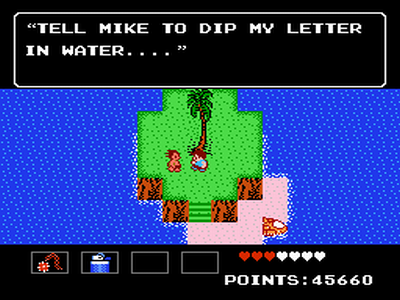
\includegraphics[width=0.48\textwidth, height=180px]{img/startropics-tell-mike.png}
        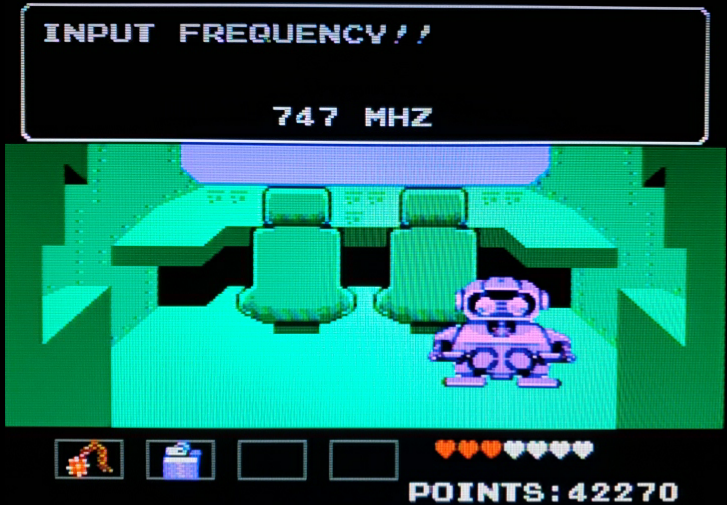
\includegraphics[width=0.48\textwidth, height=180px]{img/startropics-474.png}
        \caption{The proverbial letter can be found in Appendix \ref{apdx:letter}}
    \end{figure}

\section{Hardware}
    \todo[add]{Magnavox Odyssey}
    Odd hardware through the years:
\begin{itemize}[label=]
    \item \citegame{odyssey-simon}
          \citegame{odyssey-invasion}
          \citegame{odyssey-house}
          \citegame{odyssey-catnmouse}
          \citegame{odyssey-brainwave}
          \citegame{odyssey-percepts}
    \item \citegame{vectrex-bytemag} 
    \todo[add]{GCE Vectrex}
          \citegame{vectrex-minestorm}
          \citegame{vectrex-art}
          \citegame{vectrex-melody}
          \citegame{vectrex-animaction}
          \citegame{vectrex-spike}
    \item \citegame{sega-pico}
    \todo[add]{Sega Pico}
    \item \citegame{playdate}
    \todo[add]{Panic Playdate}
\end{itemize}

\chapter{Design \& Development\label{chap:4-dnd}}
    \todochap{DES \& DEV}

\section{The Lost AMOLED}
    \todo[add]{Preface main game concept}
The creator's names are anagrams using the first names of Daniel Handler, whom she also shares a birthday with, and his pseudonym Lemony Snicket. Chronologically, her lifetime closely matches the birth and growth of videogame technology, but was sadly cut short when she was only 32 years old.\par
Although they have been swapped and scrambled into vague equivalents, most names within this alternate universe originate from the ASOUE books \parencite{asoue}.\par
In them, there are also mentions of a secret organisation called VFD. In Snicket's world VFD stands for Volunteer Fire Department, but in ours, among other things, it means Vacuum Fluorescent Display. I found the notion of using other display type acronyms amusing, hence CRT and LED/AMOLED.\par
Beside having a name reminiscent of NES, the LED console with its CRT game came out at a time of a literal dimensional shift in computer graphics technology - a transition from 16-bit pixels on cartridges to 32-bit polygons on optical discs with all the new rendering and memory management methodologies it brought about.
\footnote{It also may or may not conveniently share a birthyear with yours truly.}

\section{The Peripheral Potpourri}
    \todo[ref,inline]{Sources on skill progression: Final Fantasy jobs, Children of Morta}

\subsection*{Paraphernalia}\hfill\textit{Paratextuality + Physicality}
    \todo[add]{manual creation}
    \todo[ref,inline]{Which manuals informed the design of mine? METAL GEAR SOLID
        % 1 SNES/SMD and 1 PS on gameplay
        % hardware notes
        }
    \nocite{tex-dnd}\nocite{tunic}

\subsection*{Preservation}\hfill\textit{Physicality + Popularity}\par
One of the most common problems that software preservation tackles is compatibility with modern systems.
After all, a binary fileset dump is not of much use without the ability to run in any capacity.
This puts CRT for the AMOLED in the precarious position when it comes to system requirements.
    \todo[add]{Hardware quirks: dials, 2 screens?}
In-world, the loading mini-game has survived thanks to the fact it was made to run on the extra circuit board whose main purpose was to maintain vital low-level hardware functionality.
    \todo[add]{How mini-game remained}
\footnote{Launch announcement confirming PS2 backwards compatibility \parencite{scea2006}.
    Inclusion of PS2 Emotion Engine and Graphics Synthesizer\cite{whirlpool}
    \todo[add]{explain PS3$\to$PS2 Backwards compatibility}}
Other remaining components are only supplemental materials: documentation and discussion in either paper of hypertext format.
This also justifies the primitive look and complexity of the mini-game.

\subsection*{Personalisation}\hfill\textit{Paratextuality + Popularity}
    \todo[add]{Interpretations and practices shaping legacy:
        cite magazine preview, web review, and forum commentary}
    \todo[ref]{Inspo for discussions on the above}

\section{The Salvaged Software}
    \todo[add]{Purpose of mini-game: Platform + player calibration}

\subsection*{Prototype}
    \todo[dev]{Polished wireframe}
\begin{figure}[ht!]
    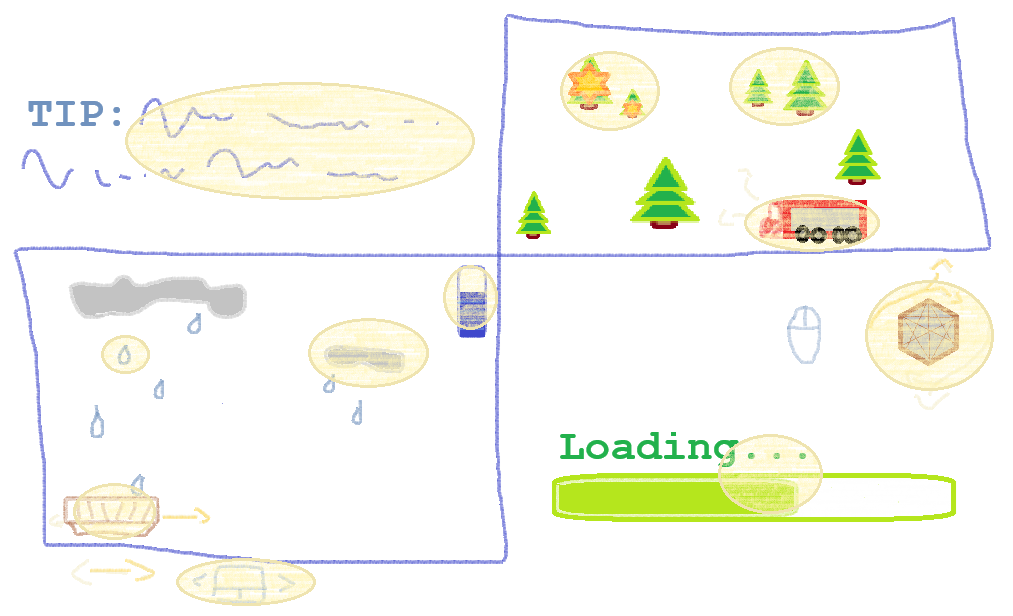
\includegraphics[width=0.8\textwidth]{img/MA-idea.png}
    \centering\caption{``Paper'' prototype}
\end{figure}
    \todo[ref,inline]{Primary sources for direction: 
        Space Invaders loading mini-game, The Sims cases}
    \todo[rtd]{Develop interface devnotes}
        screens correspond to hand placement: left hand collects water, right hand steers the truck;
        \\ controls were "canonically" separate dials and/or other analogue components;
        \\   here they are tied to a single mouse which is why each is confined to a single axis;
        \\   mouse buttons serve as pedals for the fire truck;
        \\   already seems a bit tricky to multitask, may need to automate movement;
        \\ loading bar tracks the mini-game's progress under the hood; does not sync with score increase but updates at an interval to be less obvious
        \\ shows Start when full
        \\   maybe our goal can be to have the player ignore the launch button once it appears;
        \\ My metagame score as a designer is the superfluous scoring that a player gets byond the 100\%
        \\ tips give ambiguous clues for the main game; juicier details come later on
        \\ talk aout number tweaking
    \todo[rtd]{Develop world environment devnotes}
        Two islands connected via piping, one supplies the other with water
        \\Trees at spawn over time; Four growth stages.
        \\   Saplings appear in the vicinity of fully grown trees
        \\ The bigger the tree, the more flammable it is, but generating larger clouds
        \\
        \\ Clouds float in and out of the lower frame, causing rainfall for water collection
        \\ Raindrops fall at the same speed but appear faster from larger clouds;
        \\ The larger the cloud, the higher up it is positioned
        \\ Why not wind
        \\
        \\ Firetruck 
        \\ upgrades for successful incident management;
        \\   fires extinguished $\to$ larger bucket and tank capacity
        \\   water collected    $\to$ better truck?
        \\   auto-pilot for both vehicles
        \\   auto-bucket with mostly free tank slides towards lowest raindrop, otherwise closest water tower
        \\ \nocite{flood}
        \\ what if: FLOOD (random idea) !?
    
    \todo[dev]{start screen?}
    \todo[dev]{auto-pilot  truck}
    \todo[dev]{Input prompts}
    \paragraph{Assets}
        \citetitle{crt-shader}
        \citetitle{font-adore64}
        \citetitle{kenney-1bit} for most sprites
        \citetitle{kenney-monorpg} for city backdrop tiling
        \citetitle{kenney-pixelplat} for backdrop background and pipes
    \todo[dev,noinline]{ASSET HUNT: sounds, animation?}
    
\chapter{Synthesis}
    \todochap{SYNTH}
    \todo[add]{How theory and/in practice inform/clash with each other:
        massive Stranger Things spoilers}
    \todo[end]{Revision of the 3 components}
    \todo[ref,inline]{Correlation with sources? Should be mostly unused secondary}
    \todo[end]{Provisional answer to the research question}

\chapter{Conclusion}
    \todochap{OUTRO}
    \todo[end]{Critical reflection on achievement}
    \todo[end]{Outline of implications and further research directions to build upon.}
    \todo[end,inline]{Recommended reading/playing not mentioned earlier
        Friedrich Adolf Kittler versus Marshall McLuhan on media theory
        \nocite{sicart-argo}
        \nocite{rusch}
        \nocite{dragonslair1983}
    }
\vfill
    \todo[end]{\large Final word count minus references, footnotes and appendices 
        %     456 Abstract
        %    +425   out of  400 exp. in Chapter 1
        %    +360   out of 2400 exp. in Chapter 2
        %    +135   out of 1800 exp. in Chapter 3
        %    +514   out of 1400 exp. in Chapter 4
        %           out of 1600 exp. in Chapter 5
        %           out of  400 exp. in Chapter 6
    }
\hfill\textit{\large Word count: 1436}

\renewcommand{\headrulewidth}{0pt}\newgeometry{margin=16mm}
\newpage\addcontentsline{toc}{chapter}{References}\fancyhf{}
\printbibliography[title={\LARGE Bibliography}, filter=readings]
\printbibliography[title={\LARGE Ludography},   filter =  games]
\DeclareFieldFormat{url}{\\\hspace*{-8mm}{\scriptsize\faExternalLink*}\quad\url{#1/}}
\printbibliography[title={\LARGE Assets},       filter = assets]

\newgeometry{margin=4mm}
\titleformat{\chapter}[hang]{\bfseries\LARGE\scshape}{Appendix \thechapter}{16em}{}\appendix
    \todochap{APPEND}

\chapter{Paratexts\label{apdx:paratxt}}                        
\vspace{-16mm}
\section{Manual\label{apdx:manual}}              
\begin{figure}[ht!]\centering
    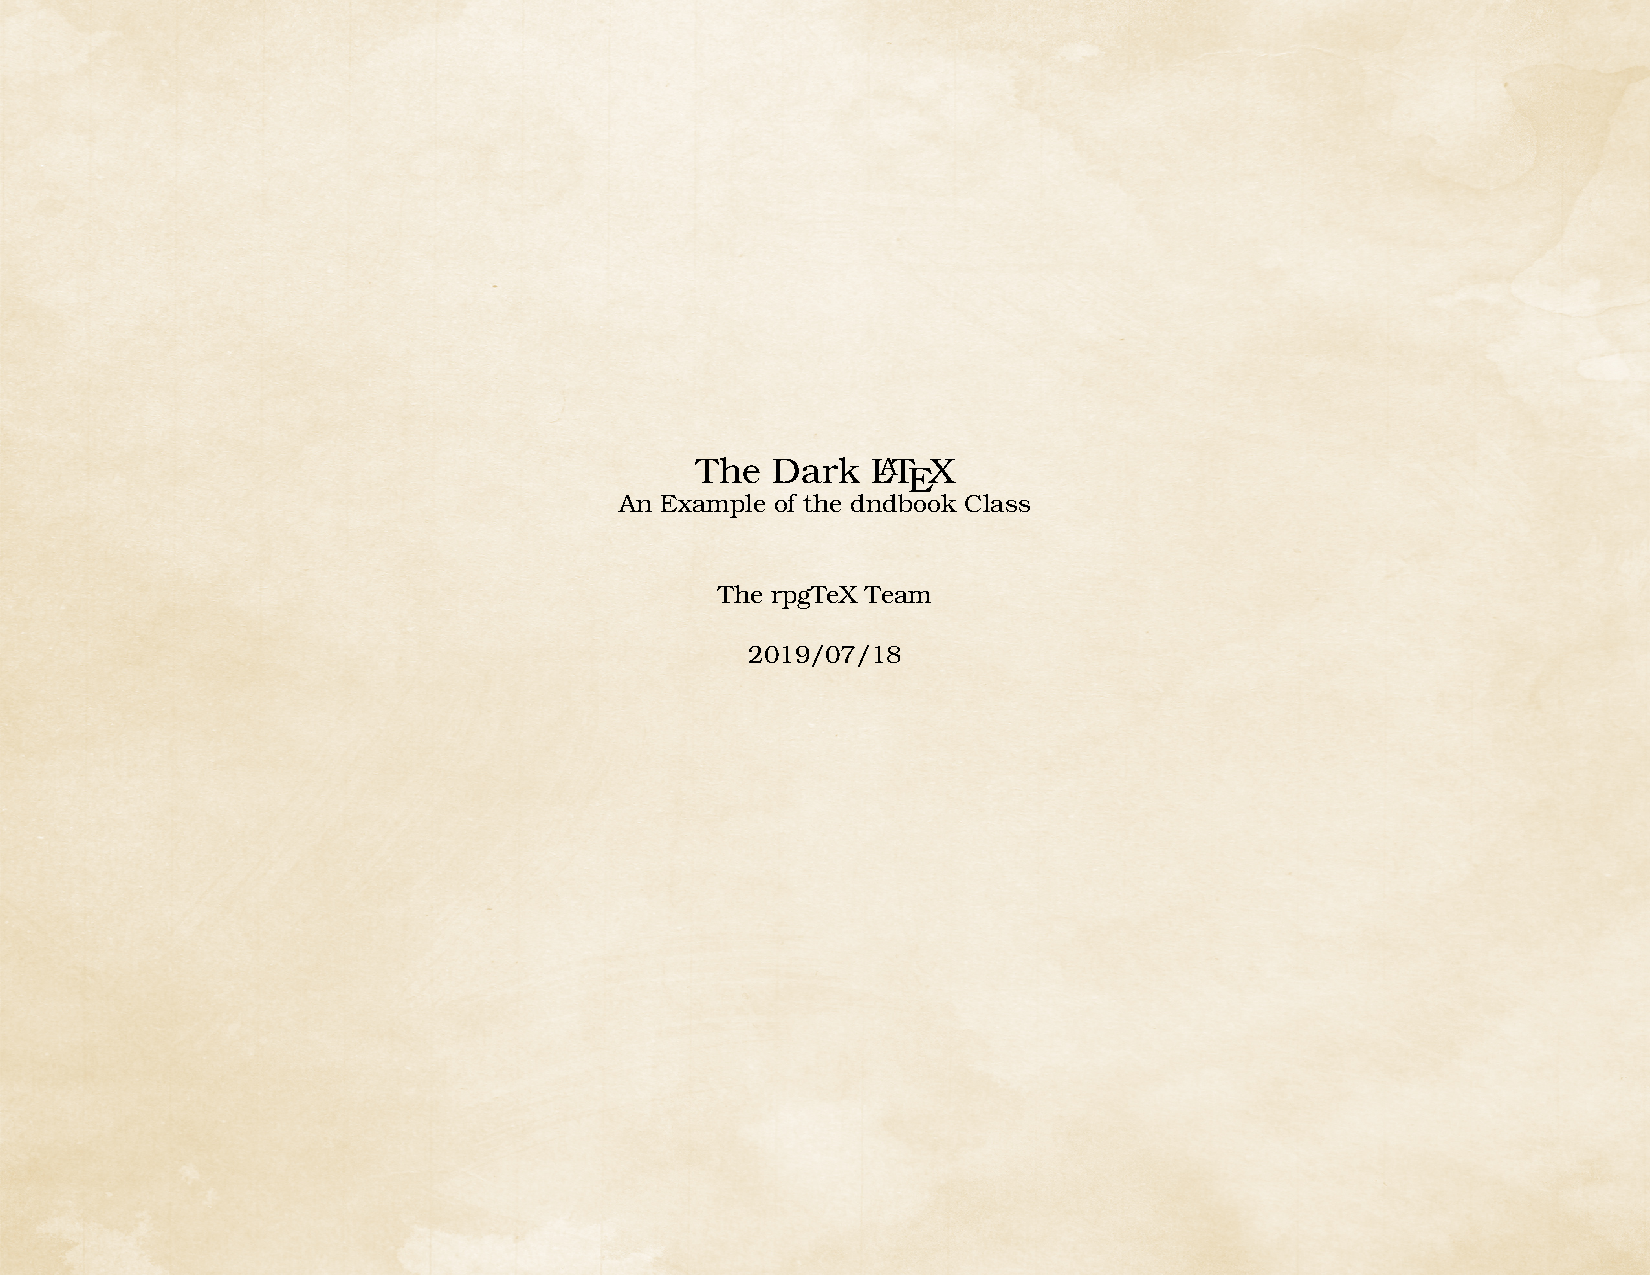
\includegraphics[page=1,width=0.48\textwidth]{man/manual.pdf}
    \includegraphics[page=2,width=0.48\textwidth]{man/manual.pdf}
    \\\vspace{2mm}
    \includegraphics[page=3,width=0.48\textwidth]{man/manual.pdf}
    \includegraphics[page=4,width=0.48\textwidth]{man/manual.pdf}
    \\\vspace{2mm}
    \includegraphics[page=5,width=0.48\textwidth]{man/manual.pdf}
    \includegraphics[page=6,width=0.48\textwidth]{man/manual.pdf}
\end{figure}
    \todo[app]{World Setting}
    Start with a quote to vibe check the world setting. 
    \\ Start telling the daily story of the common representation of the character.
    \\ Later expand on the greater causes. 
    \\ End with a semi-cliffhanger raising questions on how the worlds problems can be solved.
    \todo[app]{Factions}
    Simply title every faction than list their differentiating specs.
    \\ Their goal
    \\ Their way of doing things to reach said goal
    \\ Their social bureaucracy and hierarchy
    \\ Powers that makes them special
    \\ Their fallbacks 

    \todo[dev]{Controls}
    \todo[app]{Gameplay}
    Start with the goal of each scene/level/game.
    \\ Mention the desired gameplay loop.
    \\ Then go into detail.
    \\ Keep it basic such as, select the villager, send villager to cut trees, send back the villager to collect the timber, use banked timber to build a house via selecting the house from the building menu, this will grant you a new villager, rinse and repeat.
    \todo[app]{Campaigns
            - Mission Objectives
            - Planning/Protocol interface
            - Organising teams/squads
            - Performing actions}
    \todo[app]{Characters' Progression \& Skill trees}

\newpage\section{Articles}\vspace{-4mm}
\subsection*{A.2.1\quad Magazine preview\label{apdx:mag-art}}\vspace{-2mm}
Used \cite{tex-paper} for page layout.
\begin{figure}[ht!]\centering
    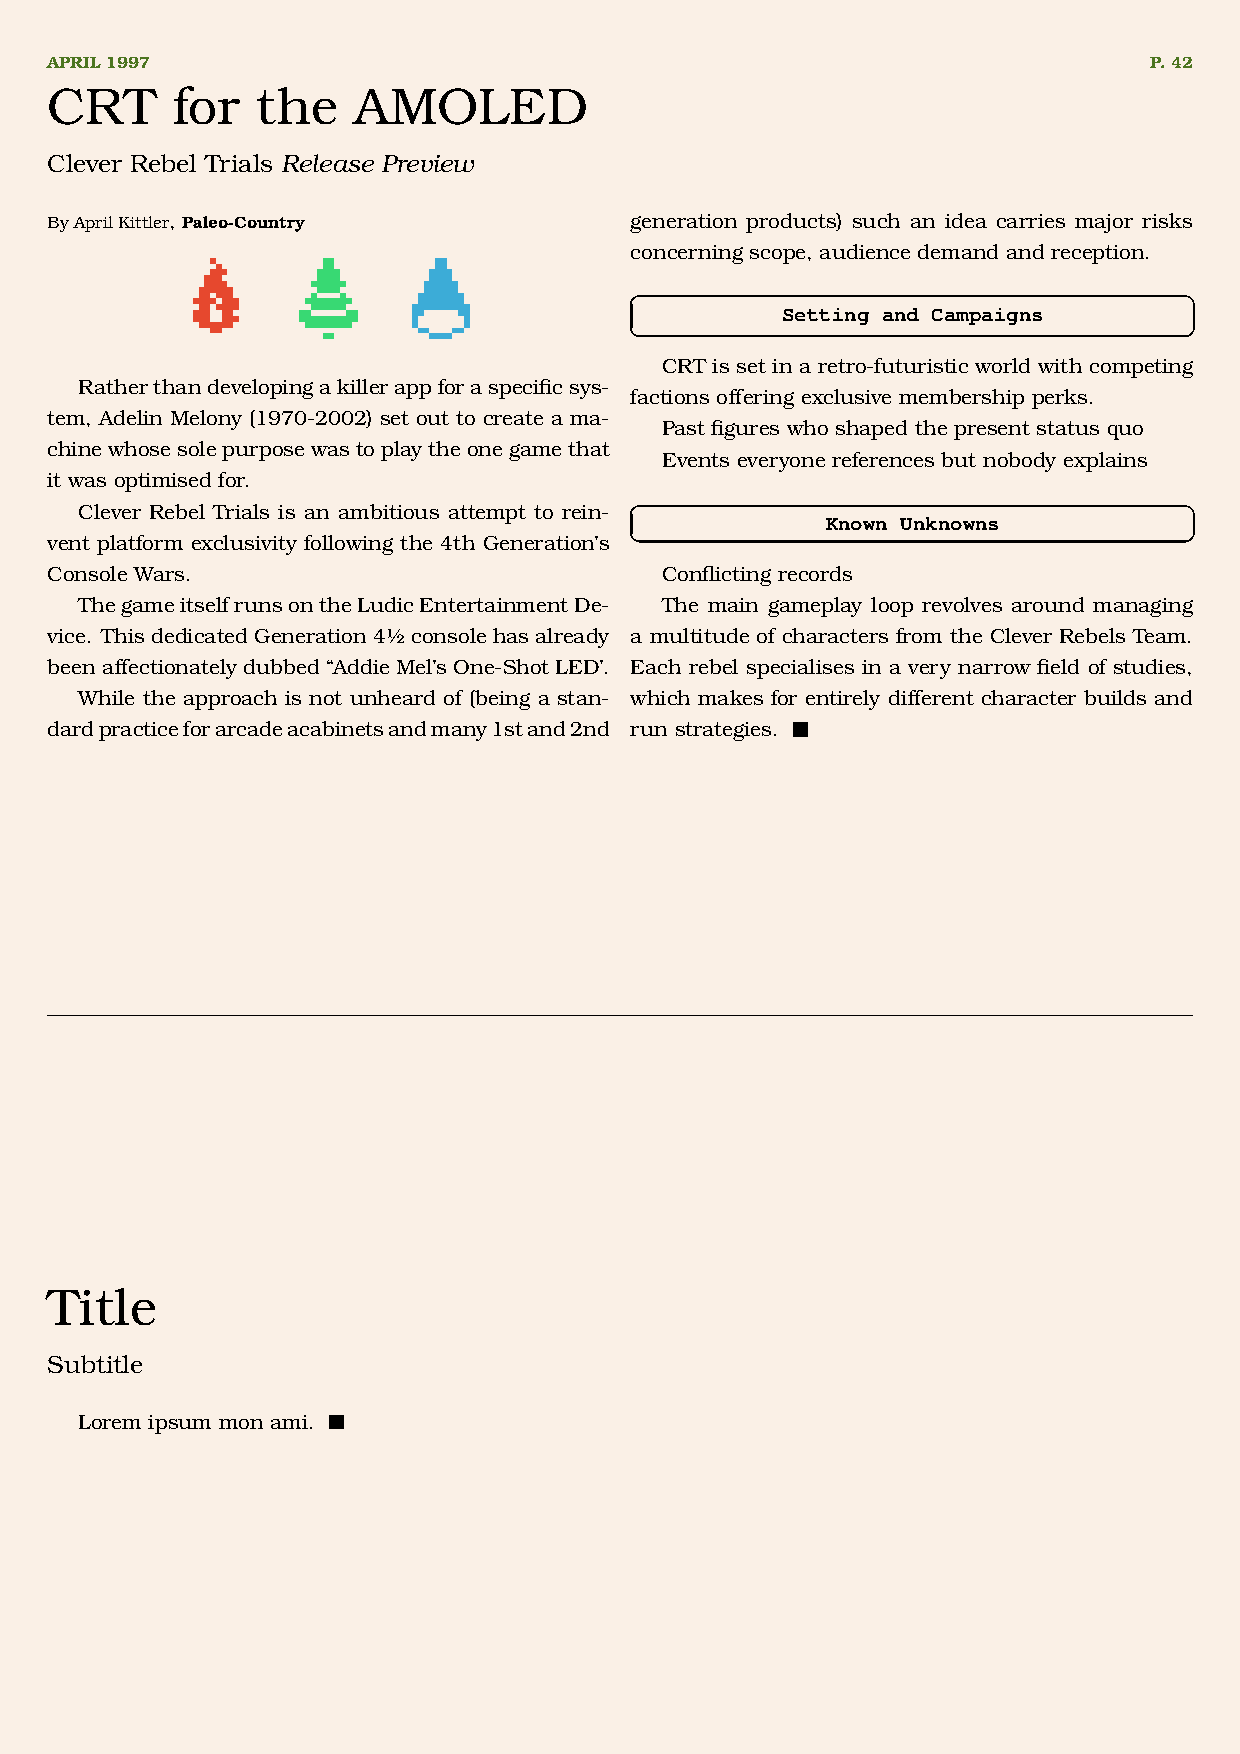
\includegraphics[scale=0.8]{mag/magazine.pdf}
    \todo[app]{Promotional article}
    \todo[app]{Interview}
\end{figure}
    \newpage
\subsection*{A.2.2 \quad Webpage review\label{apdx:web-art}}
    \todo[app]{Critical content}
    \todo[app]{About the author and tags}\newpage
\section{Message board(s)\label{apdx:msg-thr}}          
    \todo[dev]{Finish up HTML}
    \todo[app]{fill thread with user comments}

\chapter{More Media}
\begin{figure}\centering
    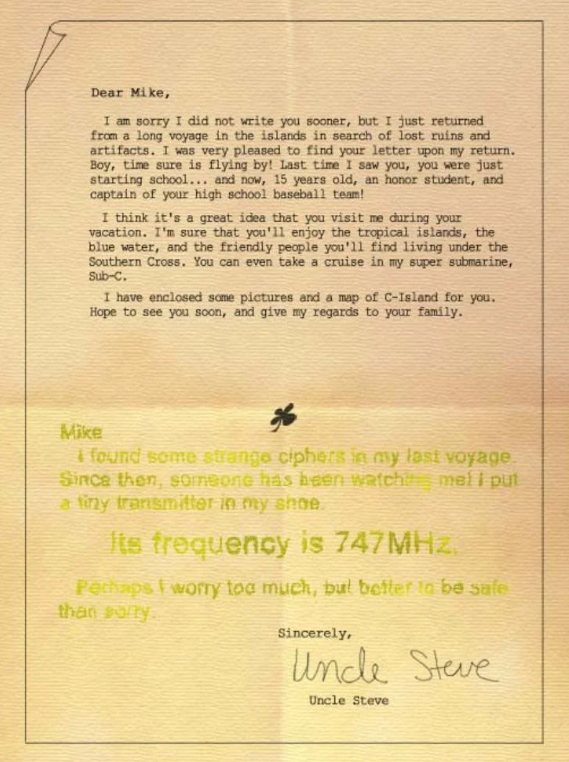
\includegraphics{img/startropics-wet-letter.png}
    \caption{\label{apdx:letter}}
\end{figure}
    \todo[ref]{Caption StarTropics letter}

    \newpage\newgeometry{margin=4mm,headheight=24mm,top=1in,bottom=1in}
    \listoftodos[\vspace{-32mm}{TO-DO List\large}\vspace{-16mm}]\pagenumbering{gobble}
\end{document}